\documentclass[12pt]{paper}
\usepackage[english]{babel}
\usepackage{indentfirst}
\usepackage{graphicx}
\usepackage{latexsym}
\usepackage{amsmath}
\usepackage{amsthm}
\usepackage{amssymb,amsfonts}
\usepackage{multicol}
\usepackage{xcolor}
\usepackage{changepage}
\usepackage{hyperref}
\usepackage{fancyhdr}
\usepackage{textcomp}
\usepackage{mathtools}
\usepackage{comment}
\usepackage[normalem]{ulem}
\usepackage{marginnote}
\usepackage[numbers,sort&compress]{natbib}
\mathtoolsset{showonlyrefs=false}

\newcommand{\ga}{\alpha}
\newcommand{\gb}{\beta}
\newcommand{\gam}{\gamma}
\newcommand{\gd}{\delta}
\newcommand{\eps}{\epsilon}
\newcommand{\veps}{\varepsilon}
\newcommand{\gz}{\zeta}
\newcommand{\gt}{\theta}
\newcommand{\gi}{\iota}
\newcommand{\gk}{\kappa}
\newcommand{\gl}{\lambda}
\newcommand{\gs}{\sigma}
\newcommand{\go}{\omega}
\newcommand{\Gam}{\Gamma}
\newcommand{\gD}{\Delta}
\newcommand{\gT}{\Theta}
\newcommand{\gL}{\Lambda}
\newcommand{\gS}{\Sigma}
\newcommand{\gO}{\Omega}

%%%%%%%%%

\newcommand{\pt}[1]{\left( #1\right)}
\newcommand{\pq}[1]{\left[ #1 \right]}
\newcommand{\pg}[1]{\left\{ #1\right\}}
\newcommand{\figref}[1]{\figurename~\ref{#1}}
\newcommand{\red}[1]{\textcolor{red}{#1}}
\newcommand{\blue}[1]{\textcolor{blue}{#1}}
\newcommand{\gray}[1]{\textcolor{gray}{#1}}
\newcommand{\wikilink}[2] { \href{#1.pdf}{#2}\,(\href{#1.tex}{edit})}

\setlength{\textheight}{20cm}
\changepage{2.5cm}{3.0cm}{-4cm}{-1.0cm}{-2cm}{-2cm}{-0.6cm}{0.5cm}{0cm}
\pagestyle{fancy}
\lhead{\bf \today}
\chead{\bf Folding kinetics and dynamics}
\rhead{EG}
\title{Folding kinetics and dynamics -- \today}
\author{EG}
\date{\today}

\begin{document}
 \maketitle
\wikilink{home}{Home}

\wikilink{research\_calculations}{Research: Calculations}

\section{Stability}\label{sec:stability}
We  calculate average and median number of contacts in native sequences, according to 
HP-model. It is measured in the units of hydrophobic energy per $kT$.
\begin{figure}[h!]
  \centering
  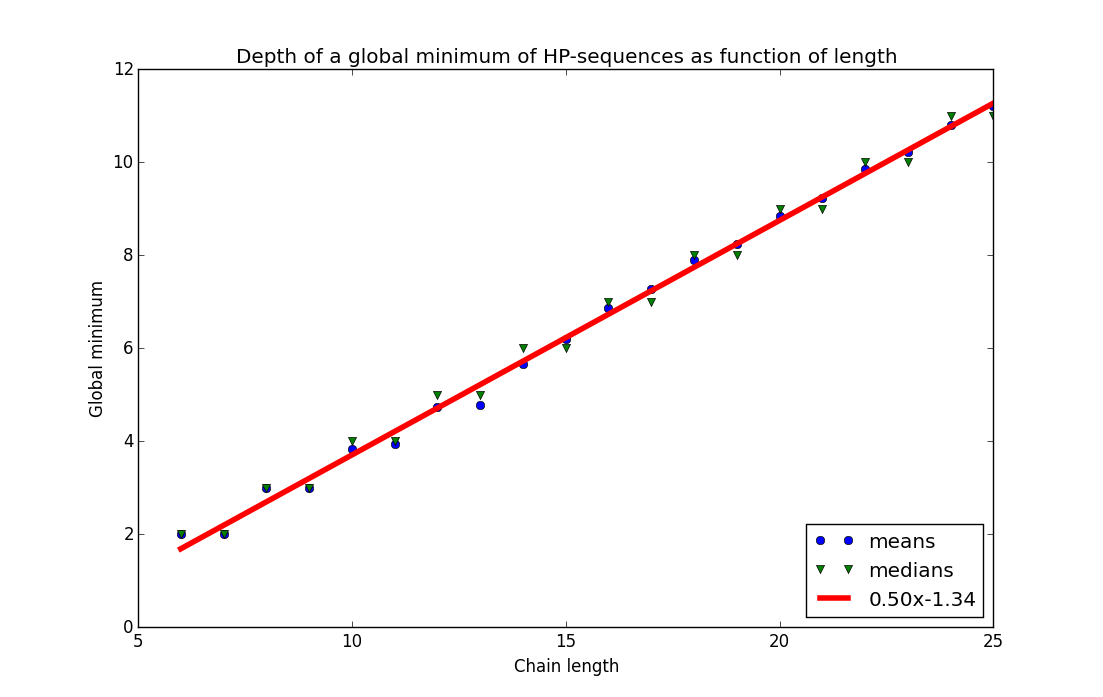
\includegraphics[width=0.85\textwidth]{pictures/hp-depth-length.png} 
  \caption{Depth of the energy well is measured in the units of $e_h=E_h/kT$, where $e_h$ is an 
energy of one hydrophobic contact per $1kT$.}
  \label{fig:hp-depth-length}
\end{figure}
From \cite{Ghosh2009} it follows that free energy is composed of two terms: the enthalpy and 
entropy of the molecular interactions and $\gD G_0=\gD H_0-T\gD S_0$ and conformational entropy 
$\gD G_c=-T\gD S_c=kTN ln z$. $N$ here is a chain length and $z$ is a number of rotational 
freedoms.

Fitting a line on a figure \ref{fig:hp-depth-length} to the HP-model minimums yields the following 
dependency for the energy well depth (per $1kT$):
\begin{equation}
\gD G_0= -kNe_h-be_h= -0.5Ne_h +1.34e_h
\end{equation} 
where $N$ is a chain length and $e_h$ is an absolute value of the energy 
of one hydrophobic contact.
And full free energy of folding will be (per $1kT$):
\begin{equation}
 \gD G = -bNe_h -be_h+N\ln z
\end{equation} 

\section{Kinetcis}
There's a theory of protein folding introduced by Ghosh and Dill in a series of papers 
\cite{Ghosh2010,Dill2011} and more. It is based on simple equilibrium thermodynamics and leads to 
the following conclusion regarding chain length distribution:
  \begin{equation}\label{eq:lnk}
   \ln k_f=16.15-1.28 \sqrt{N}
  \end{equation} 
Which in turn predicts the following dependency of the rate constants:
\begin{figure}[h!]
  \centering
  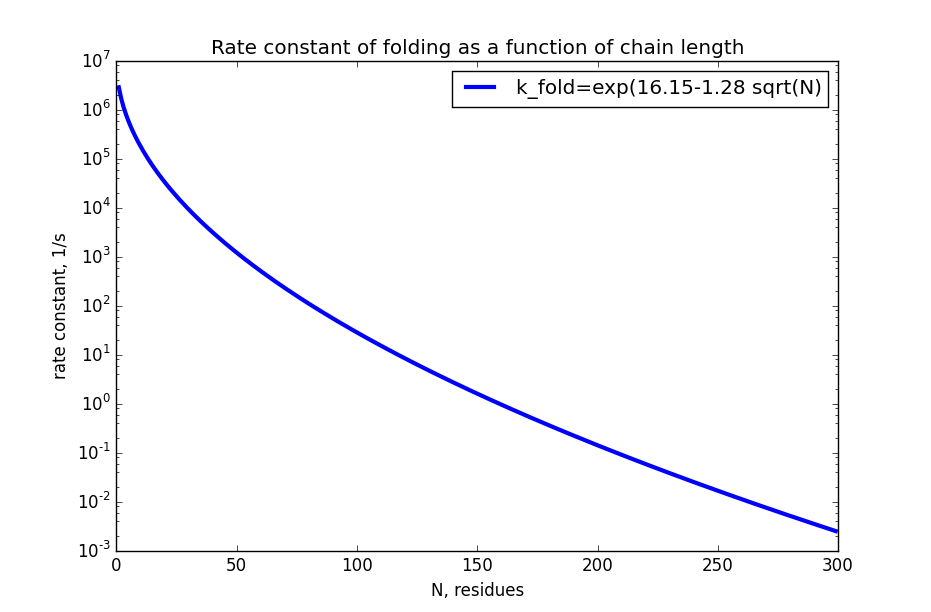
\includegraphics[width=0.85\textwidth]{pictures/k_fold_N.png} 
  \caption{}
  \label{fig:k_fold_N}
\end{figure}
While it is likely that model fails at the short sequences, we can use it for a crude estimation 
of the folding and unfolding rates of the short HP-polymers. Though there's no real way to test if 
our results are true.
This model suggests that the \textit{folding} rate constants would be the following for some short 
chains:
  \begin{itemize}
   \item $k_f(10)=2\cdot 10^5$
   \item $k_f(20)=3\cdot 10^4$
   \item $k_f(30)=0.9\cdot 10^4$
  \end{itemize}

Folding and unfolding rate constants relate to each other and free energy of folding.
\begin{equation}
 \ln\pt{\frac{k_f}{k_u}}=\ln K=-\gD G/kT
\end{equation} 
From the section \ref{sec:stability}, if $\gD G_0$ follows law from fig.\ref{fig:hp-depth-length}  
it follows that:
\begin{equation}
\ln k_f-\ln k_u=\gD G_0/kT-N\ln z%=\frac{1}{z^N}\exp(-\gD G_0/kT)
\end{equation} 
which gives
\begin{equation}
\ln k_u = \ln k_f -\gD G_0/kT+N\ln z 
\end{equation} 
Substituting $\ln k_f $ from equation \eqref{eq:lnk} and fitted $\gD G_0$ we get:
\begin{equation}
\ln k_u = 16.15-1.28 \sqrt{N} -bNe_h -be_h+N\ln z
\end{equation} 
Therefore
\begin{equation}
k_u = \frac{1}{z^N}exp(16.15-1.28 \sqrt{N} -bNe_h -be_h)
\end{equation} 
This gives the following dependencies for $k_u$ and $k_f$: see fig.\ref{fig:k_unf_N}
\begin{figure}[h!]
  \centering
  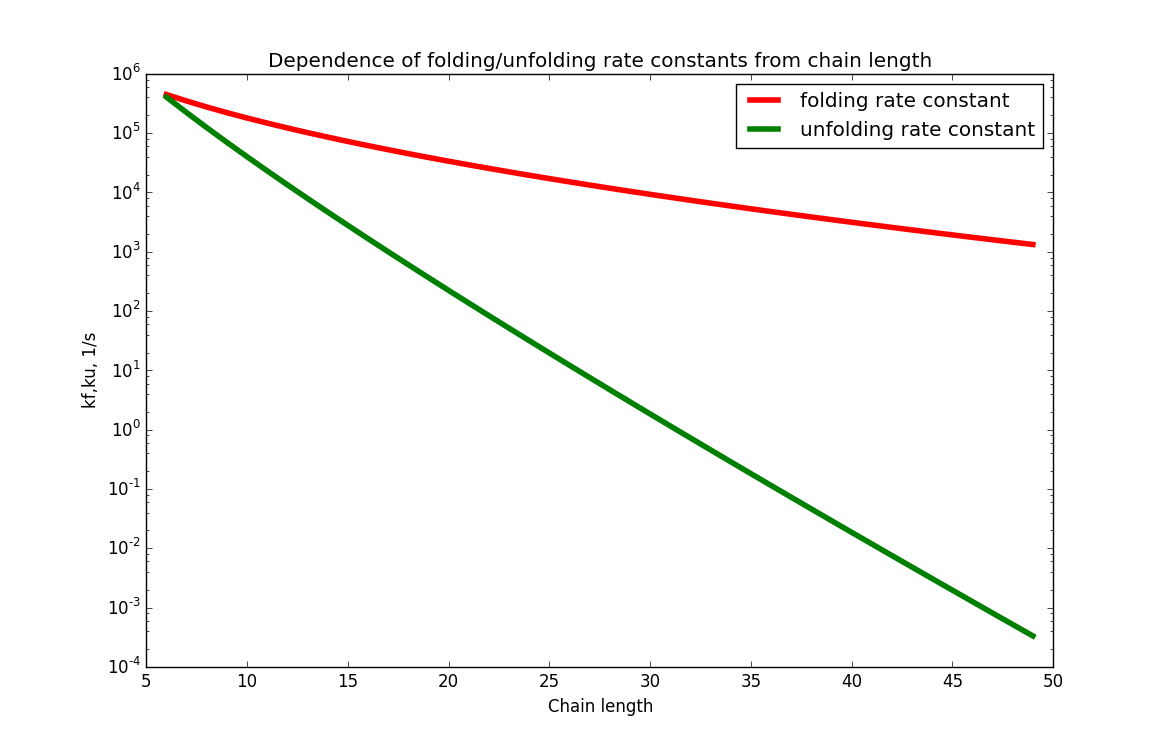
\includegraphics[width=0.95\textwidth]{pictures/kf-ku.png} 
  \caption{Folding and unfolding rates as a function of chain length. $e_h=1.5,z=1.5$ This numbers 
are chosen so that equilibrium constant is around $10^2-10^4$ when chain lengths are short (around 
15-30), see figure \ref{fig:K}}
  \label{fig:k_unf_N}
\end{figure}
\begin{figure}[h!]
  \centering
  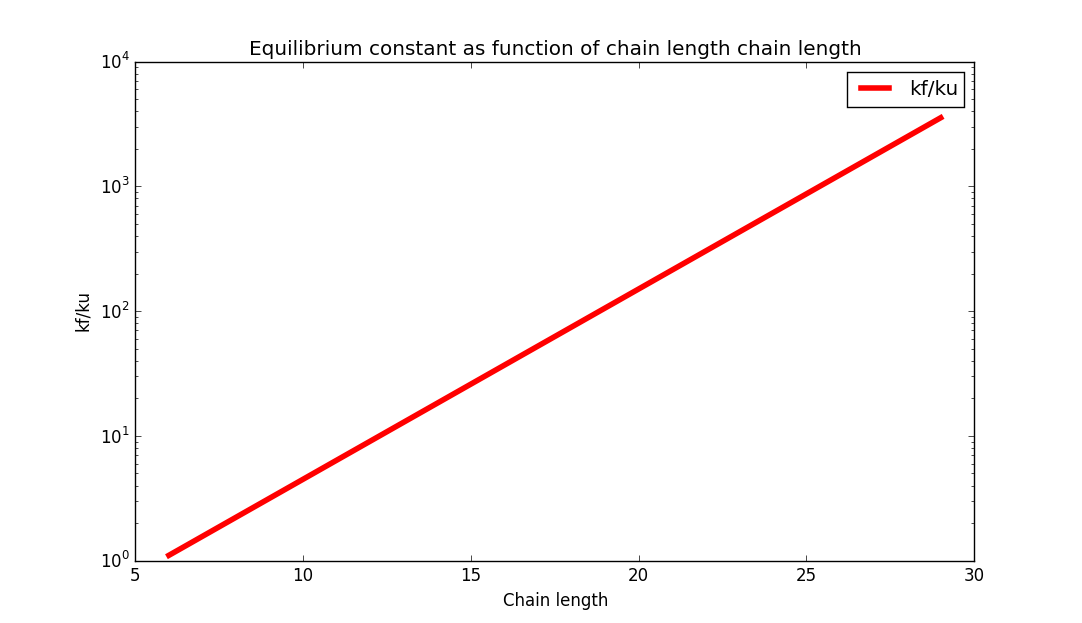
\includegraphics[width=0.95\textwidth]{pictures/K.png} 
  \caption{Equilibrium constant as a function of chain length. $e_h=1.5,z=1.5$ This numbers are 
chosen so that equilibrium constant is around 
$10^2-10^4$ when chain lengths are short (around 15-30)}
  \label{fig:k_unf_N}
\end{figure}

  \bibliography{/data/research/31.mendeleyBibtex/library}
  \bibliographystyle{unsrt}
\end{document}
